\chapter{Perhitungan Aritmatika Pendukung}

\noindent Lampiran ini berisikan contoh perhitungan yang terjadi di dalam model yang dikembangkan dalam penelitian. Perhitungan menggunakan data yang sederhana untuk memberikan pemahaman intuitif terhadap cara kerja model. 

\section{Operasi Konvolusi}
\noindent Pada arsitektur Attention U-net operasi konvolusi menggunakan padding agar output yang dihasilkan tetap memiliki dimensi sama dengan input. Padding adalah penambahan nilai nol di sekitar tepi citra input. Hal ini dilakukan agar setiap piksel pada citra input memberikan kontribusi pada hasil konvolusi sehingga informasi spasial tidak hilang. Berikut adalah gambaran kerja operasi konvolusi dengan tambahan padding disekitar citra input.

\begin{figure}[H]
	\centering
	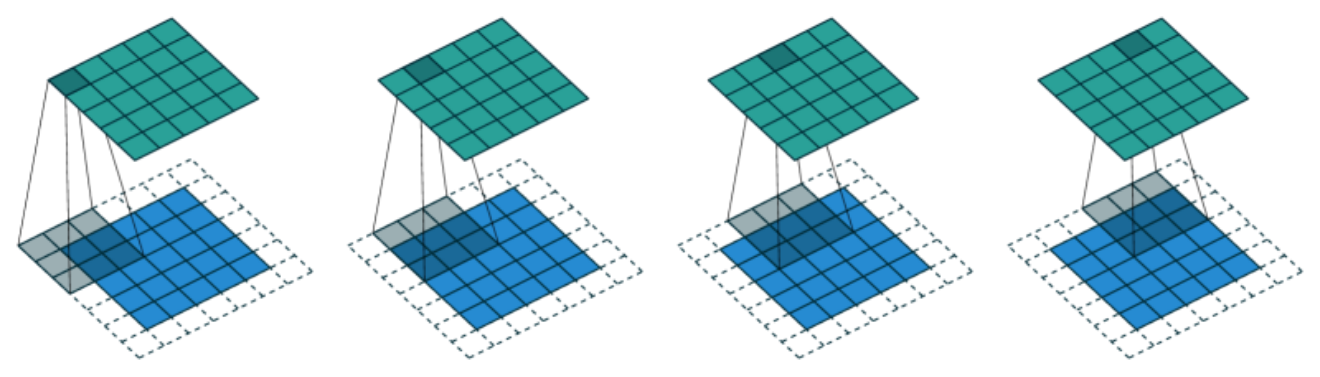
\includegraphics[scale=.4]{gambar/lampiran/stride.png}
\end{figure}

\noindent Selanjutnya contoh perhitungan dari operasi konvolusi menggunakan data yang sederhana:

\begin{figure}[H]
	\centering
	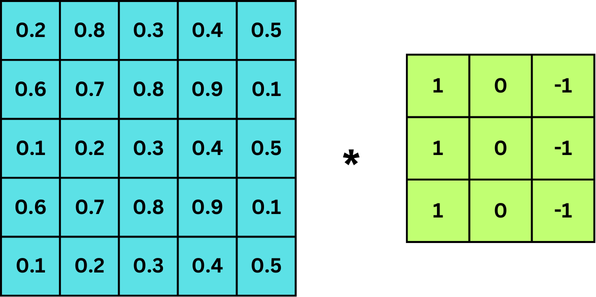
\includegraphics[scale=.3]{gambar/lampiran/konvolusi.png}
\end{figure}

\noindent Anggap kita punya sebuah input citra input 5 x 5 dengan filter edge detection 3 x 3.

\begin{figure}[H]
	\centering
	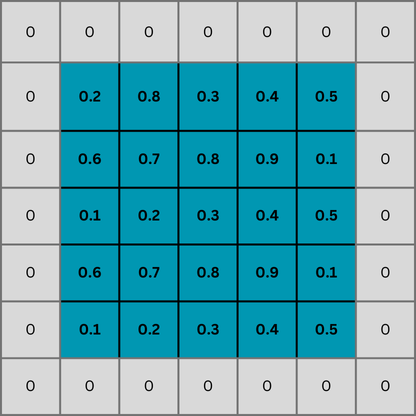
\includegraphics[scale=.3]{gambar/lampiran/padding.png}
\end{figure}

\noindent Langkah pertama adalah penambahan piksel bernilai 0 disekitar citra.


\begin{figure}[H]
	\centering
	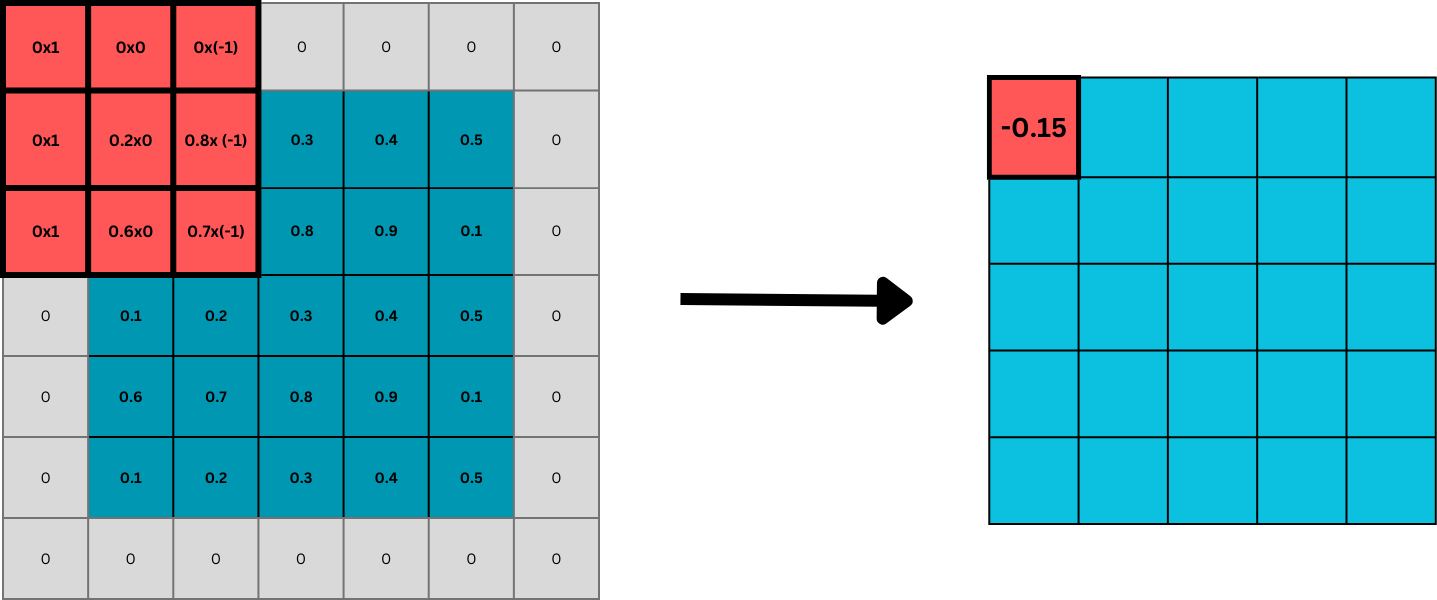
\includegraphics[scale=.3]{gambar/lampiran/posisi-awal.png}
\end{figure}
\noindent Setelah itu filter akan dilakukan perhitungan konvolusi di atas input untuk menghasilkan output di titik \([0,0]\) dengan detail sebagai berikut: 

(1 * 0) + (0 * 0) + (-1 * 0) + (1 * 0) + (0 * 0.2) + (-1 * 0.8) + (1 * 0) + (0 * 0.6) + (-1 * 0.7) = -1.5


\begin{figure}[H]
	\centering
	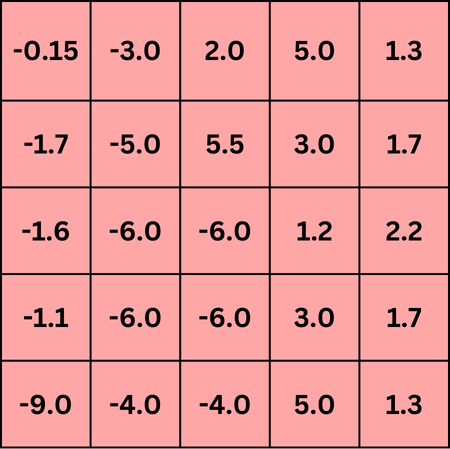
\includegraphics[scale=.3]{gambar/lampiran/hasil-konvolusi.png}
\end{figure}

\noindent Setelah semua bagian input dilakukan perhitungan konvolusi, akan menghasilkan output seperti di atas.

\section{Pooling}


\noindent Operasi pooling yang digunakan pada attention U-net adalah max-pooling. Max-pooling mengambil nilai maksimum dari setiap wilayah yang dilewati oleh filter.  Ukuran filter yang umum digunakan adalah 2x2, dengan stride (langkah) sebesar 2.  Artinya, filter akan bergerak 2 langkah secara horizontal dan vertikal pada setiap iterasi. berikut adalah contoh dari penerapan max-pooling pada input sederhana 4 x 4 dan filter yang digunakan 2 x 2.

\begin{figure}[H]
	\centering
	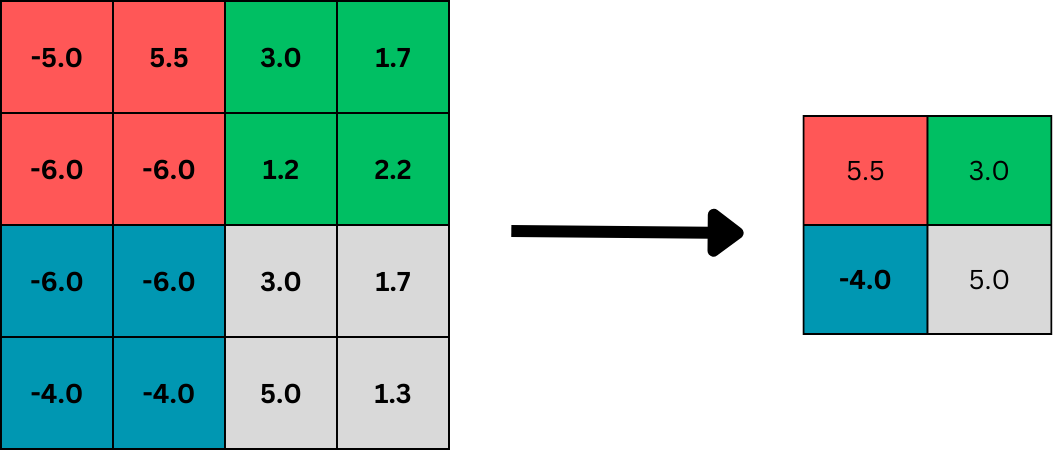
\includegraphics[scale=.3]{gambar/lampiran/pooling.png}
\end{figure}

\noindent Pada contoh diatas daerah yang dilewati filter 2 x 2 diambil nilai paling tinggi untuk menjadi nilai pada output.

\section{Transpose Konvolusi}

\noindent Transpose konvolusi menggunakan filter untuk menghasilkan peningkatan resolusi peta fitur hasil \textit{down-sampling}. Pada Attention U-net filter transpose konvolusi diterapkan pada output dengan stride 2. Contoh penerapan pada data sederhana adalah sebagai berikut:

\begin{figure}[H]
	\centering
	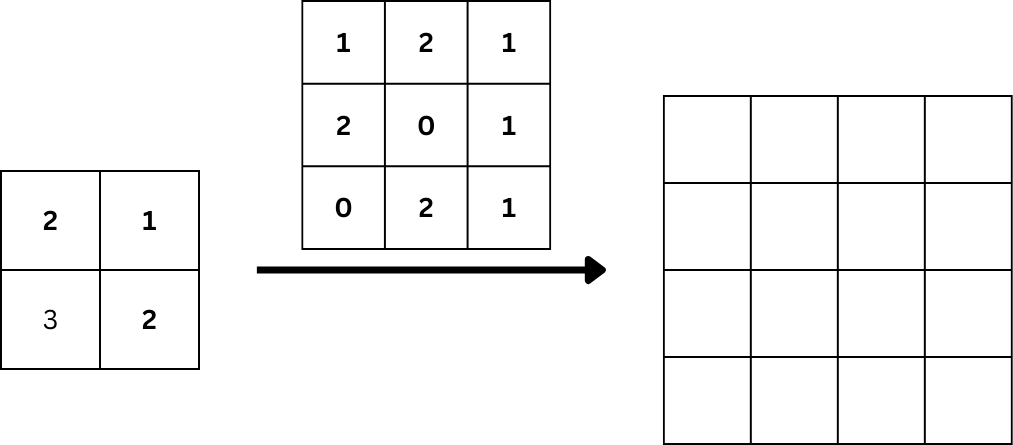
\includegraphics[scale=.3]{gambar/lampiran/dekonv-1.png}
\end{figure}

\noindent Anggap kita punya peta fitur 2 x 2 yang akan ditingkatkan resolusinya menjadi 4 x 4 dengan filter 3 x 3.

\begin{figure}[H]
	\centering
	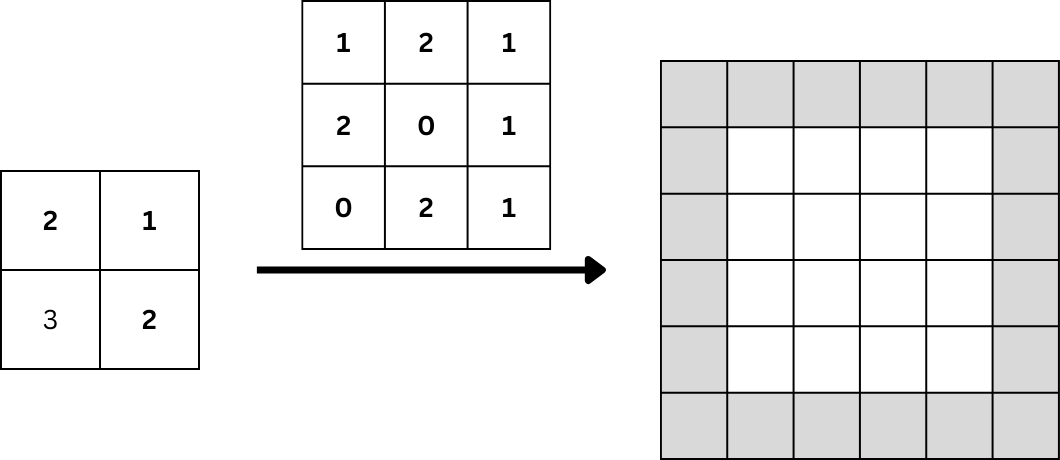
\includegraphics[scale=.3]{gambar/lampiran/dekonv-2.png}
\end{figure}

\noindent Langkah pertama adalah penambahan padding disekitar output agar operasi konvolusi bisa dilakukan.

\begin{figure}[H]
	\centering
	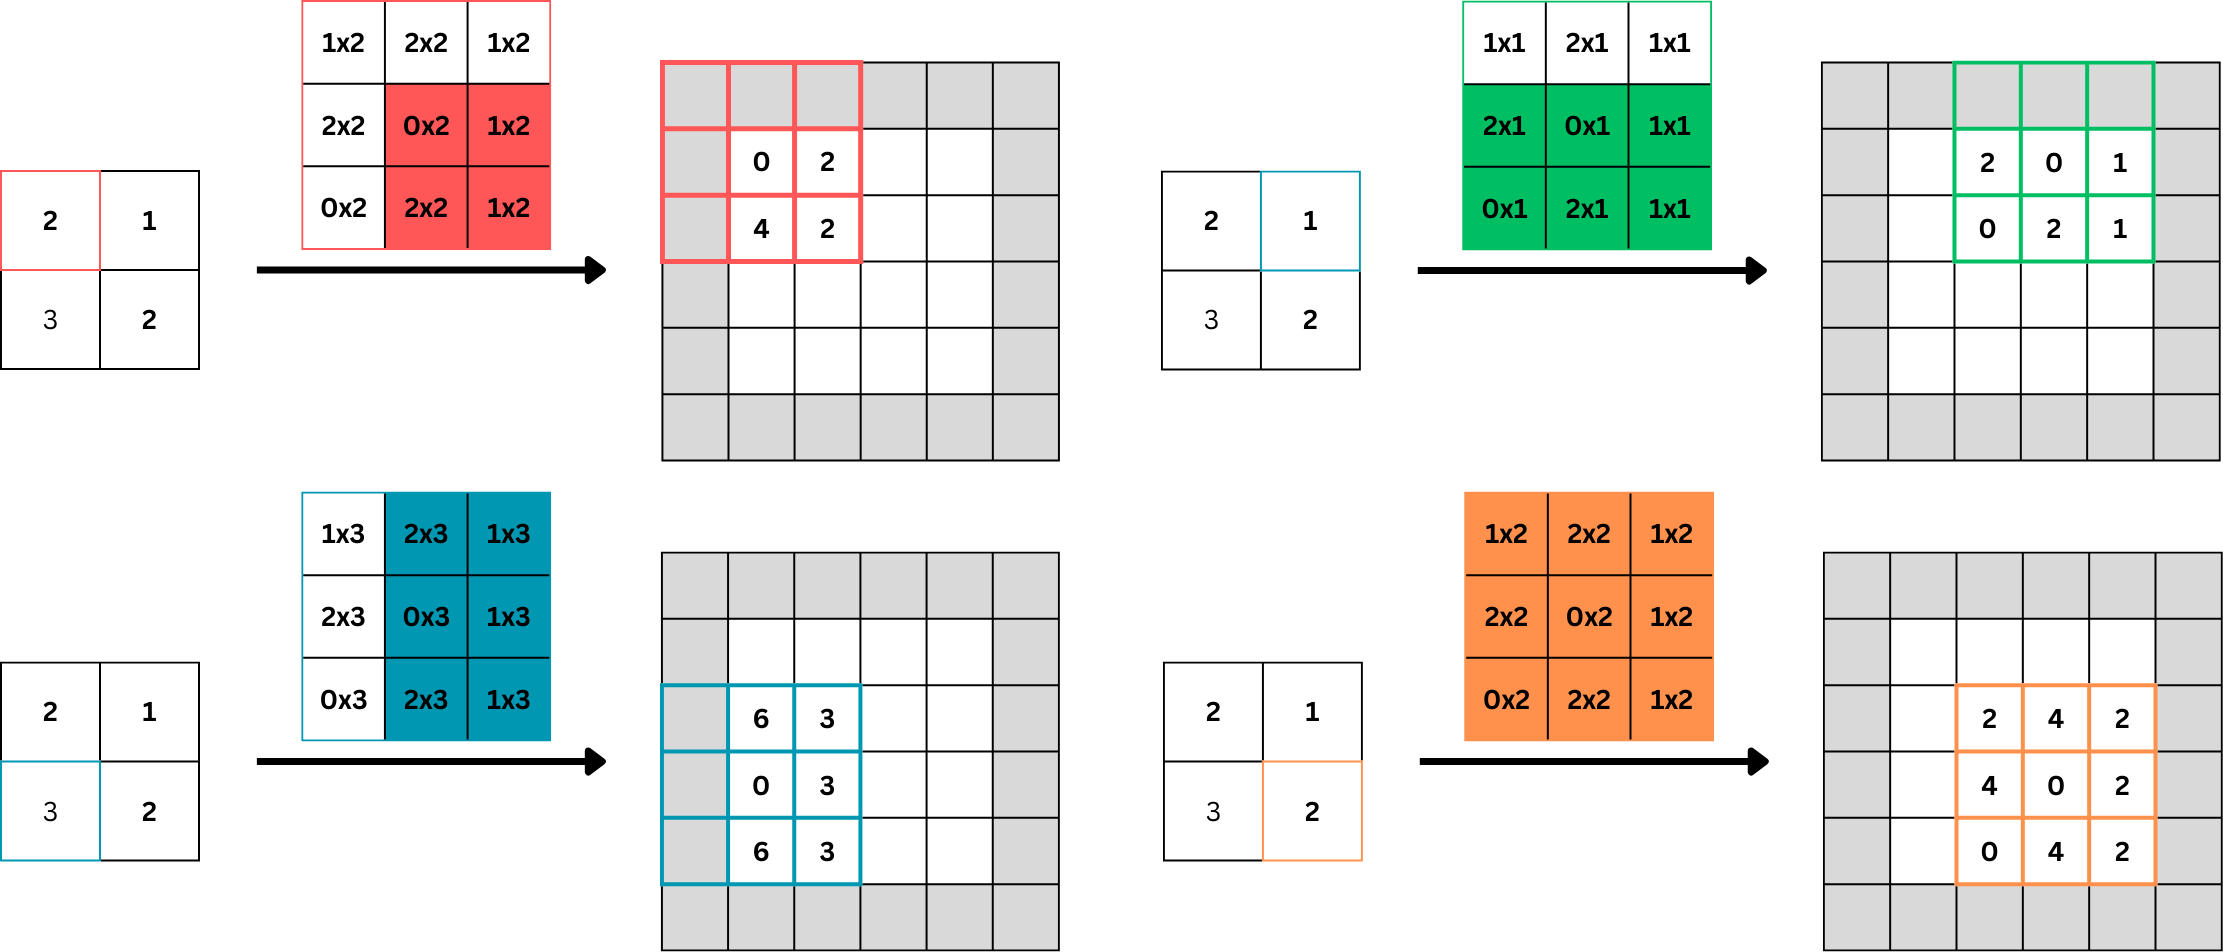
\includegraphics[scale=.2]{gambar/lampiran/dekonv-full.png}
\end{figure}

Selanjutnya input akan diambil dan dikalikan dengan setiap nilai yang ada pada filter. Area padding dihiraukan.

\begin{figure}[H]
	\centering
	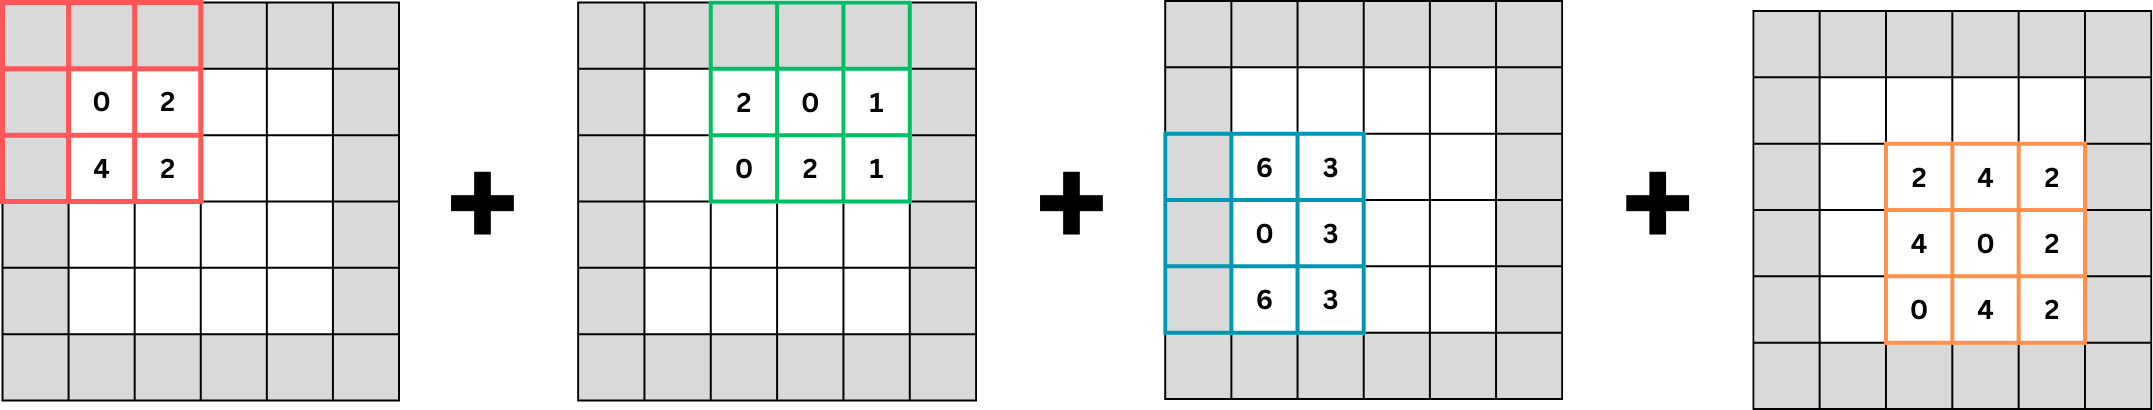
\includegraphics[scale=.3]{gambar/lampiran/dekonv-7.png}
\end{figure}

Kemudian hasil perkalian yang ada pada setiap area output akan dijumlahkan.

\begin{figure}[H]
	\centering
	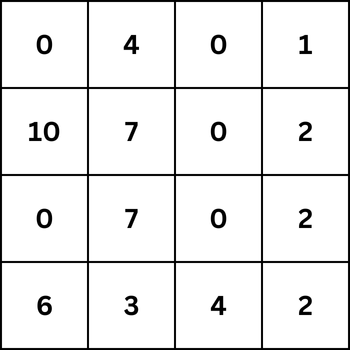
\includegraphics[scale=.3]{gambar/lampiran/dekonv-8.png}
\end{figure}

%Terakhir are padding dihilangkan sehingga kita mendapatkan output 4 x 4 seperti yang diinginkan.

\section{Fungsi Aktivasi}

\begin{figure}[H]
	\centering
	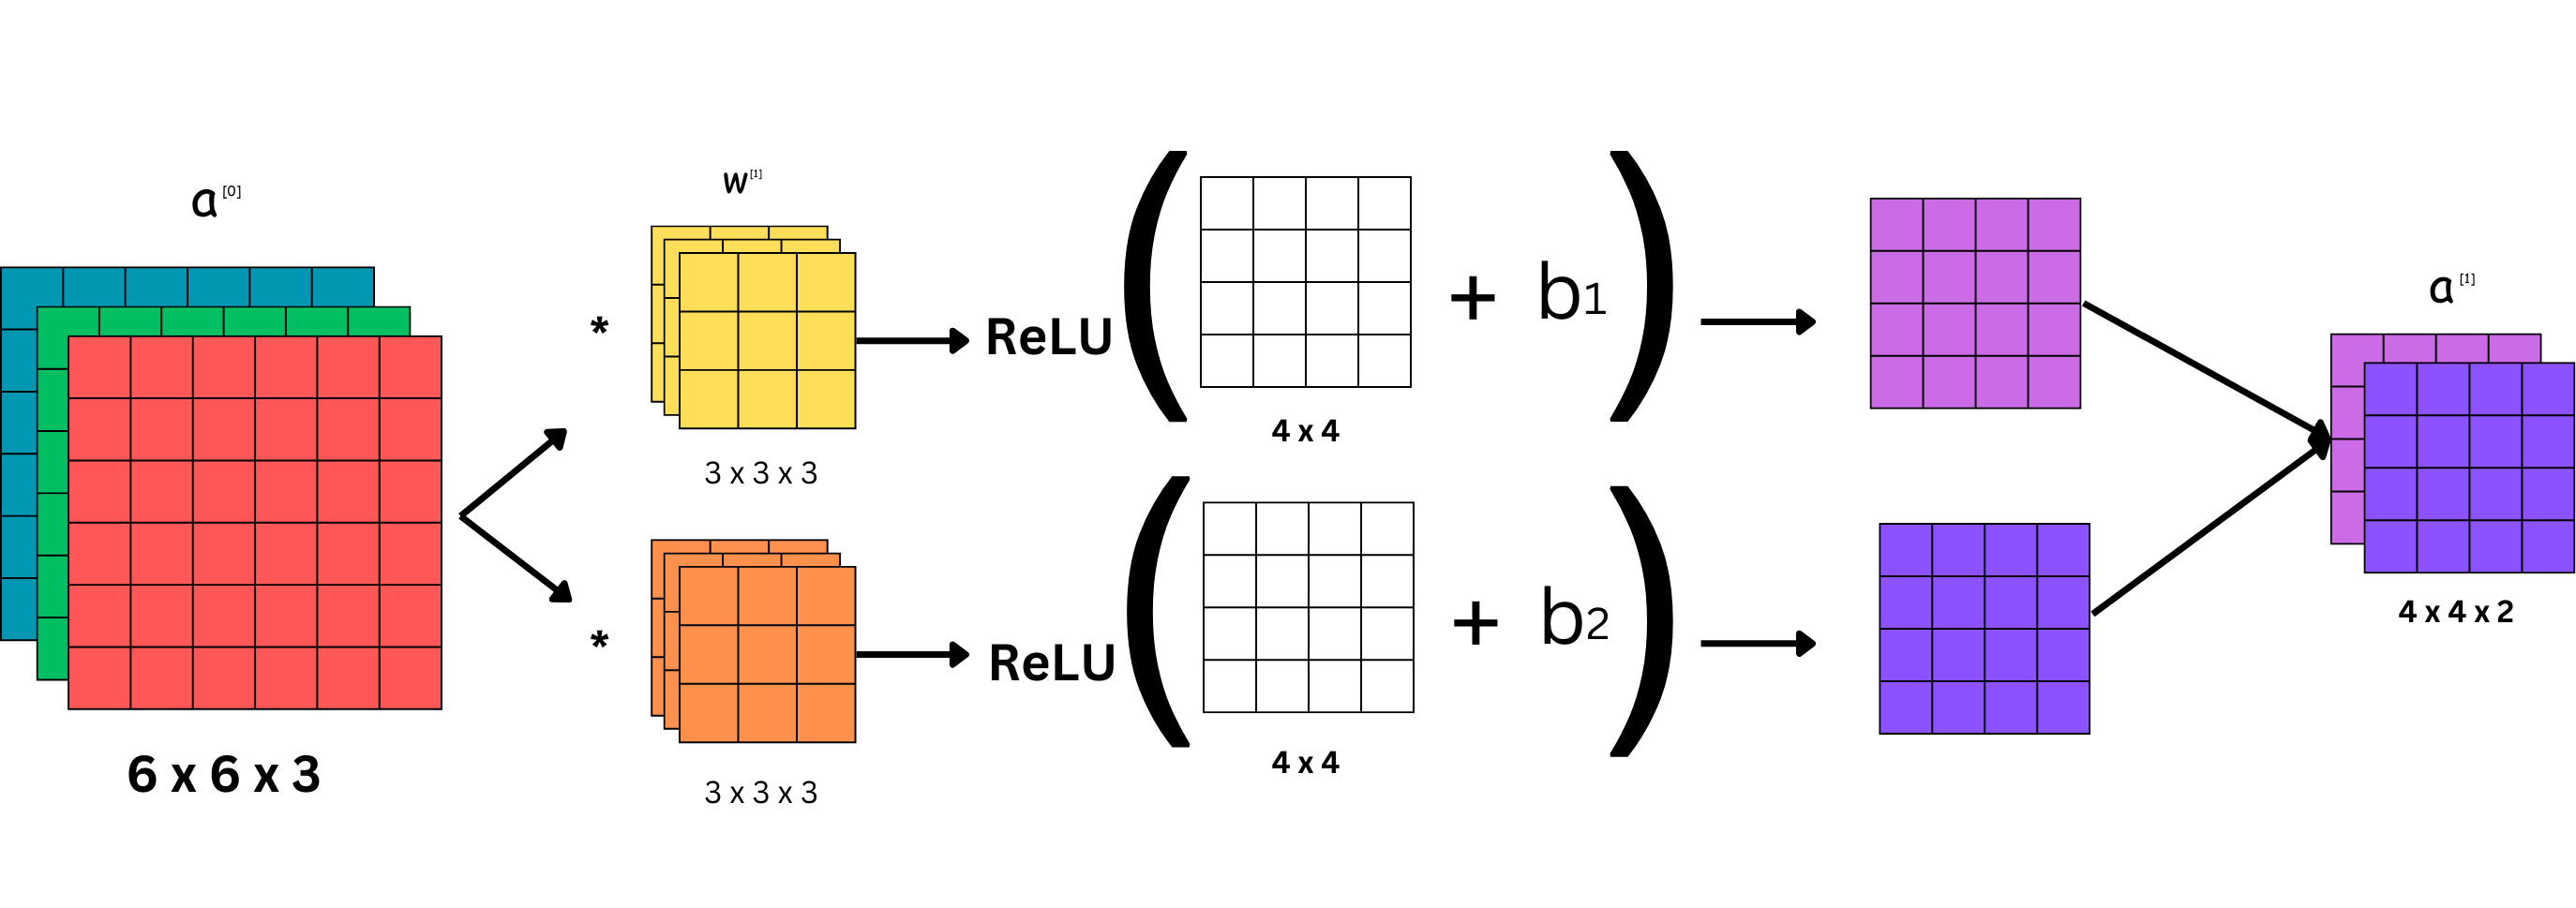
\includegraphics[scale=.2]{gambar/lampiran/feed-fwrd.png}
\end{figure}

\noindent Gambar diatas merupakan contoh sebuah layer konvolusi. Setelah dihasilkan peta fitur, jaringan akan menambahkan bias pada peta fitur tersebut untuk mengatur nilai output dari neuron. Kemudian, fungsi aktivasi ReLU (Rectified Linear Unit) diterapkan pada setiap elemen feature map. ReLU mengubah semua nilai negatif menjadi nol, dan mempertahankan nilai positif apa adanya. Berikut adalah contoh dari penerapan ReLU pada peta fitur.

\begin{figure}[H]
	\centering
	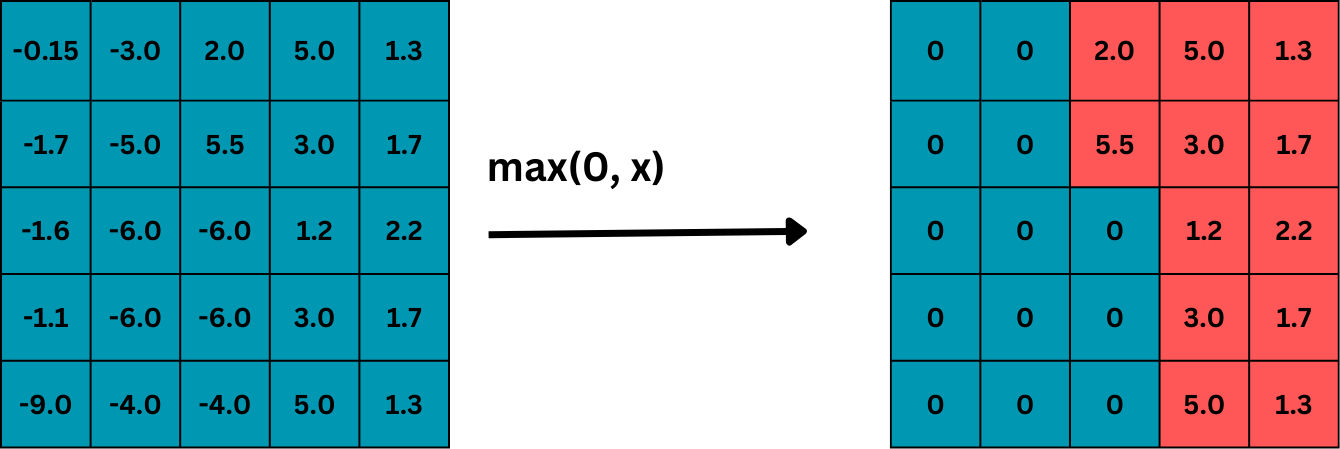
\includegraphics[scale=.2]{gambar/lampiran/fungsi-relu.png}
\end{figure}

ReLU mengubah setiap nilai negatif menjadi 0 dan mempertahankan nilai positif apa adanya. Sebagai contoh, untuk elemen pertama (-0.15), karena nilainya negatif, maka ReLU(-0.15) = 0.  Untuk elemen ketiga (2.0), karena nilainya positif, maka ReLU(2.0) = 2.0.

\noindent Fungsi aktivasi sigmoid memiliki cara kerja yang sama dengan ReLu, dimana fungsi ini akan diterapkan pada setiap elemen dari peta fitur. berikut adalah contoh perhitungan dari fungsi aktivasi sigmoid pada peta fitur yang sama dengan perhitungan pada contoh ReLU:

\[
\sigma(-0.15) = \frac{1}{1 + e^{0.15}} \approx 0.46257
\]

\[
\sigma(-3.0) = \frac{1}{1 + e^{3.0}} \approx 0.04743
\]

\[
\sigma(2.0) = \frac{1}{1 + e^{-2.0}} \approx 0.88080
\]

\[
\sigma(5.0) = \frac{1}{1 + e^{-5.0}} \approx 0.99331
\]

\[
\sigma(1.3) = \frac{1}{1 + e^{-1.3}} \approx 0.78583
\]



\section{Evaluasi}
 
 \noindent Pada Attention U-net, evaluasi yang digunakan untuk melihat kemampuan model dalam memprediksi objek adalah Interseption ove Union (IoU) dan Dice Similarity Coefficient (DSC). Beirikut ini adalah contoh perhitungan evaluasi model.
 
 \begin{figure}[H]
 	\centering
 	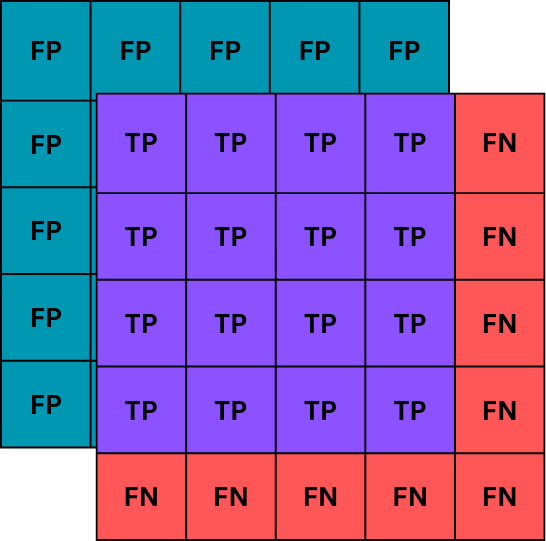
\includegraphics[scale=.2]{gambar/lampiran/prediksi.png}
 \end{figure}    
 
 \noindent Anggap kita punya kotak biru (ground truth) yang mewakili objek sebenarnya dan kotak merah (prediksi) yang merupakan prediksi model tentang lokasi dan ukuran objek. True positive (TP) merupakan area tumpang tindih antara kotak biru dan kotak merah, merupakan prediksi benar. False positive (FP) area kotak merah yang tidak tumpang tindih dengan kotak biru, merupakan prediksi yang salah. False negative (FN) area kotak biru yang tidak tumpang tindih dengan kotak merah, merupakan area objek yang tidak terdeteksi model.    
 
  \begin{figure}[H]
 	\centering
 	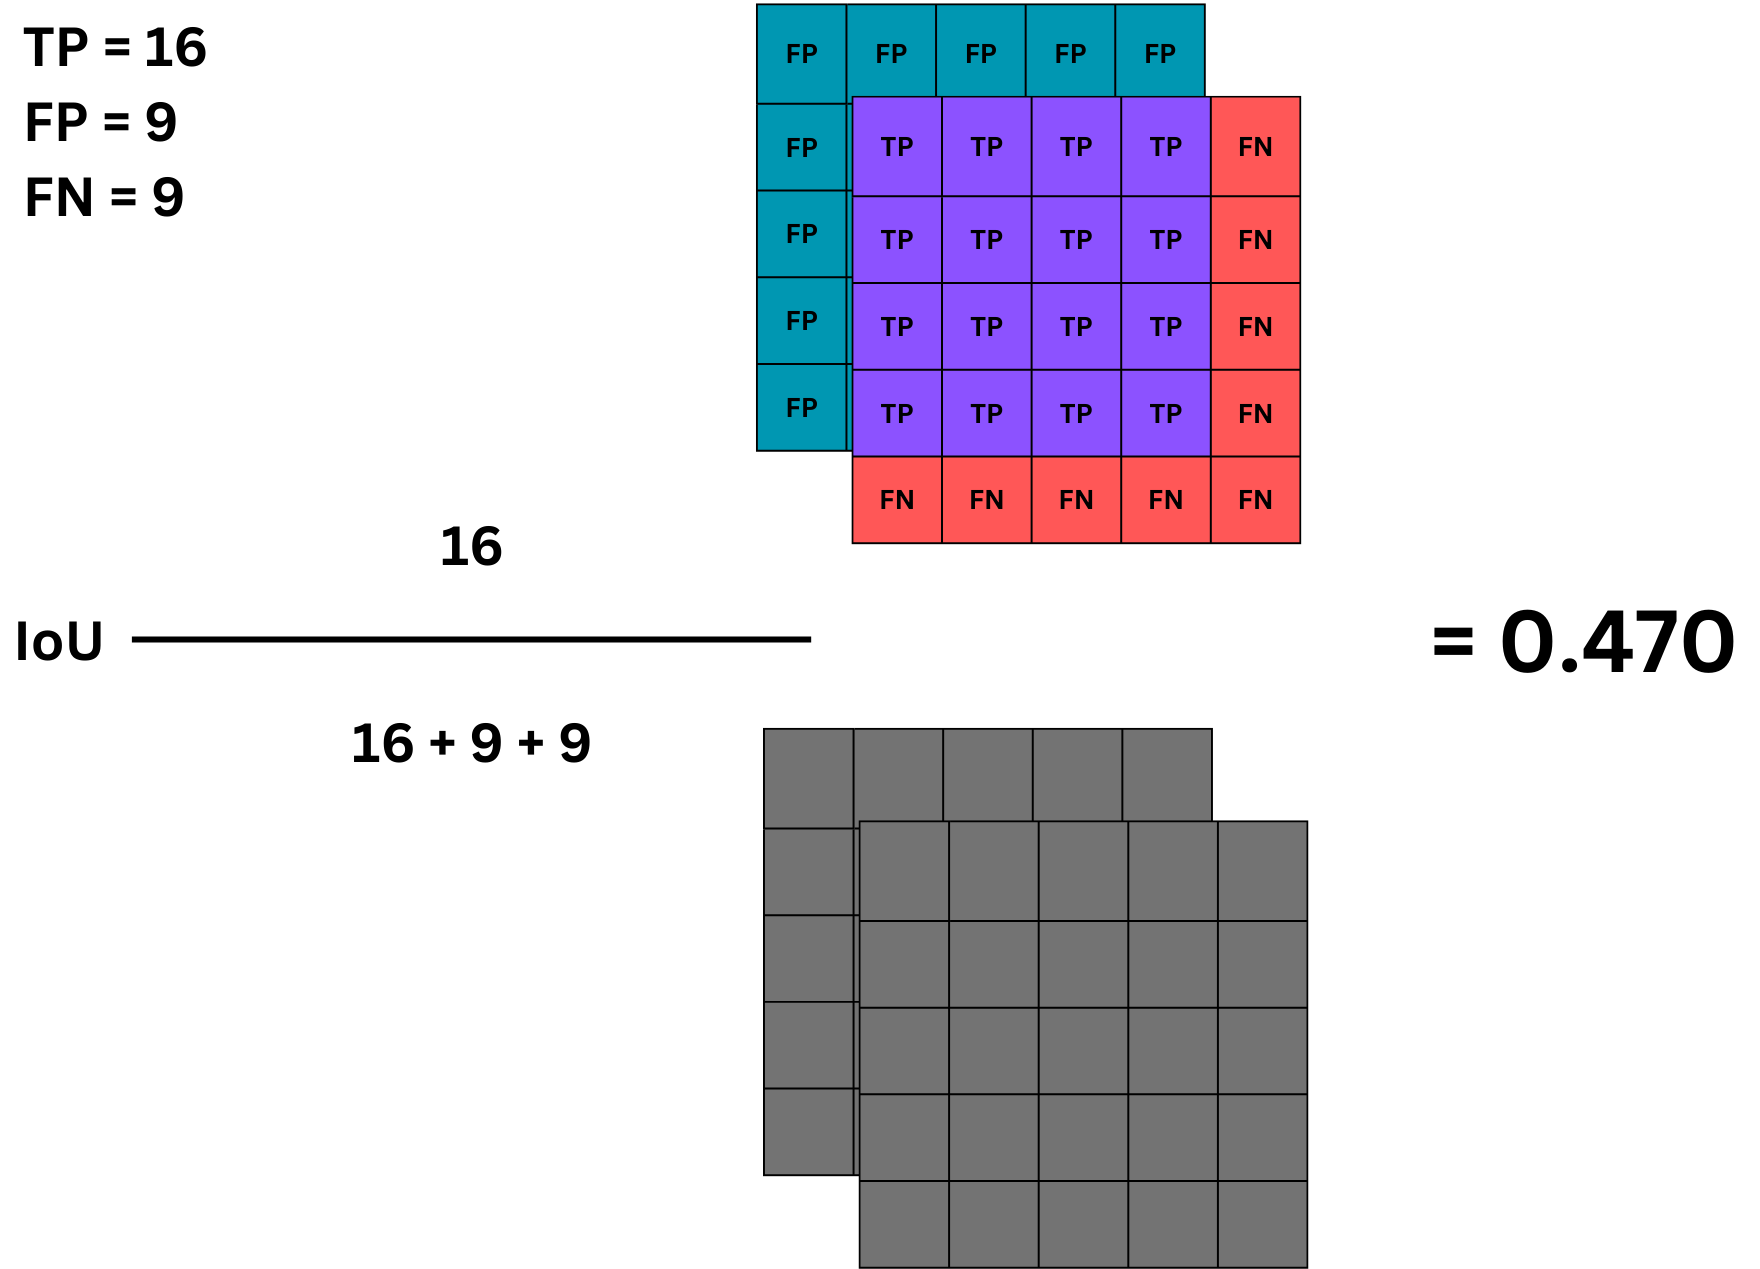
\includegraphics[scale=.2]{gambar/lampiran/IoU.png}
 \end{figure} 
 
 IoU dihitung dengan membagi luas area tumpang tindih (TP) dengan luas gabungan dari kedua kotak (TP + FP + FN). Begitu juga dengan DSC membagi dua kali area tumpang tindih (2TP) dengan luas gabungan (2TP + FP FN). 
 

%\chapter{Hasil Pengamatan} \label{lampiranD}
%\noindent Lampiran hasil pengamatan berisikan dengan \textit{logbook} selama pengamatan, citra objek, keluaran algoritma, skrip pengolahan data dengan Python, dan dokumentasi selama pengamatan.
    %\section{\textit{Logbook} Pengamatan}
     %\noindent Lorem ipsum dolor sit amet, consectetur adipiscing elit, sed do eiusmod tempor incididunt ut labore et dolore magna aliqua. Ut enim ad minim veniam, quis nostrud exercitation ullamco laboris nisi ut aliquip ex ea commodo consequat. Duis aute irure dolor in reprehenderit in voluptate velit esse cillum dolore eu fugiat nulla pariatur. Excepteur sint occaecat cupidatat non proident, sunt in culpa qui officia deserunt mollit anim id est laborum.
    %\section{Objek pada Citra Pengamatan}
    %\noindent Lorem ipsum dolor sit amet, consectetur adipiscing elit, sed do eiusmod tempor incididunt ut labore et dolore magna aliqua. Ut enim ad minim veniam, quis nostrud exercitation ullamco laboris nisi ut aliquip ex ea commodo consequat. Duis aute irure dolor in reprehenderit in voluptate velit esse cillum dolore eu fugiat nulla pariatur. Excepteur sint occaecat cupidatat non proident, sunt in culpa qui officia deserunt mollit anim id est laborum

    %\section{Dokumentasi Pengamatan}
  %\noindent Lorem ipsum dolor sit amet, consectetur adipiscing elit, sed do eiusmod tempor incididunt ut labore et dolore magna aliqua. Ut enim ad minim veniam, quis nostrud exercitation ullamco laboris nisi ut aliquip ex ea commodo consequat. Duis aute irure dolor in reprehenderit in voluptate velit esse cillum dolore eu fugiat nulla pariatur. Excepteur sint occaecat cupidatat non proident, sunt in culpa qui officia deserunt mollit anim id est laborum

%\chapter{Program} \label{lam:lampiran_a}
%\begin{lstlisting}[language=Python]
%import numpy as np

%def incmatrix(genl1,genl2):
 %   m = len(genl1)
  %  n = len(genl2)
   % M = None #to become the incidence matrix
    %VT = np.zeros((n*m,1), int)  #dummy variable

    %#compute the bitwise xor matrix
    %M1 = bitxormatrix(genl1)
 %   M2 = np.triu(bitxormatrix(genl2),1)

  %  for i in range(m-1):
   %     for j in range(i+1, m):
    %        [r,c] = np.where(M2 == M1[i,j])
     %       for k in range(len(r)):
      %          VT[(i)*n + r[k]] = 1;
       %         VT[(i)*n + c[k]] = 1;
        %        VT[(j)*n + r[k]] = 1;
         %       VT[(j)*n + c[k]] = 1;

          %      if M is None:
           %         M = np.copy(VT)
            %    else:
             %       M = np.concatenate((M, VT), 1)

              %  VT = np.zeros((n*m,1), int)

  %  return M
%\end{lstlisting}

%\chapter{Grafik Tambahan} \label{lampiran B}
 %\noindent Lorem ipsum dolor sit amet, consectetur adipiscing elit, sed do eiusmod tempor incididunt ut labore et dolore magna aliqua. Ut enim ad minim veniam, quis nostrud exercitation ullamco laboris nisi ut aliquip ex ea commodo consequat. Duis aute irure dolor in reprehenderit in voluptate velit esse cillum dolore eu fugiat nulla pariatur. Excepteur sint occaecat cupidatat non proident, sunt in culpa qui officia deserunt mollit anim id est laborum
